%; whizzy chapter -dvi
% -initex iniptex -latex platex -format platex -bibtex jbibtex -fmt fmt
% 以上 whizzytex を使用する場合の設定。
 
%     Tokyo Debian Meeting resources
%     Copyright (C) 2012 Junichi Uekawa
%     Copyright (C) 2011, 2015 Nobuhiro Iwamatsu

%     This program is free software; you can redistribute it and/or modify
%     it under the terms of the GNU General Public License as published by
%     the Free Software Foundation; either version 2 of the License, or
%     (at your option) any later version.

%     This program is distributed in the hope that it will be useful,
%     but WITHOUT ANY WARRANTY; without even the implied warranty of
%     MERCHANTABILITY or FITNESS FOR A PARTICULAR PURPOSE.  See the
%     GNU General Public License for more details.

%     You should have received a copy of the GNU General Public License
%     along with this program; if not, write to the Free Software
%     Foundation, Inc., 51 Franklin St, Fifth Floor, Boston, MA  02110-1301 USA

%  preview (shell-command (concat "evince " (replace-regexp-in-string "tex$" "pdf"(buffer-file-name)) "&"))

%%ここからヘッダ開始。

\documentclass[mingoth,a4paper]{jsarticle}
\usepackage{monthlyreport}
% 日付を定義する、毎月変わります。
\newcommand{\debmtgyear}{2017}
\newcommand{\debmtgmonth}{9}
\newcommand{\debmtgdate}{16}
% started from zero:
% (let ((year 2013) (month 7)) (+ (* (- year 2005) 12) month -1))
\newcommand{\debmtgnumber}{155}

% Needed to import pandoc-generated LaTeX documents.
% See https://stackoverflow.com/questions/40438037/tightlist-error-using-pandoc-with-markdown
\providecommand{\tightlist}{%
  \setlength{\itemsep}{0pt}\setlength{\parskip}{0pt}}

% tikz picture の為のマクロ設定
\usepackage[dvipdfmx]{graphicx}
\usepackage{tikz}

\begin{document}

\begin{titlepage}
\thispagestyle{empty}
% タイトルページ:編集必要な部分は最初のマクロに飛ばすこと

\vspace*{-2cm}
第\debmtgnumber{}回 東京エリア Debian 勉強会資料\\
\hspace*{-2cm}

\includegraphics{image2012-natsu/dotdeb.pdf}\\
\hfill{}\debmtgyear{}年\debmtgmonth{}月\debmtgdate{}日

% ここはアップデートすること
% 全角文字にしないとフォントのサイズが合わないので注意
\rotatebox{10}{\fontsize{30}{30} {\gt keysign、POMERA }}\\

\vspace*{-2cm}
\hfill{}
\includegraphics[height=6cm]{image200502/openlogo-nd.eps}
\end{titlepage}

\newpage

\begin{minipage}[b]{0.2\hsize}
 \definecolor{titleback}{gray}{0.9}
 \colorbox{titleback}{\rotatebox{90}{\fontsize{80}{80} {\gt デビアン勉強会} }}
\end{minipage}
\begin{minipage}[b]{0.8\hsize}
\hrule
\vspace{2mm}
\hrule
\begin{multicols}{2}
\tableofcontents
\end{multicols}
\vspace{2mm}
\hrule
\end{minipage}

\dancersection{最近のDebian関連のミーティング報告}{杉本 典充}

\subsection{第153回東京エリアDebian勉強会}

2017年8月19日(土)に東銀座にある朝日ネット様をお借りして、第153回東京エリアDebian勉強会を開催しました。参加者は9名でした。

発表は、青木さんとやまねさんによる「debconf17参加報告」でした。

debconf17のwebサイトは以下URLで公開しており、発表の多くをビデオで見ることができます。

\url{https://debconf17.debconf.org/}

参加報告では、会場になったカナダ モントリオールの大学の話やイベントの雰囲気、debianに関する議論、参加した発表の概要説明や感想、補足説明がありました。

\begin{itemize}
\item The Machine\footnote{\url{https://debconf17.debconf.org/talks/206/}}
\item debianパッケージのメンテナーをそのパッケージのオーナーとみなす雰囲気があるようだが実際はそのようなことはない。patch welcomeであるし、メンテナンスできる人であれば任せることもある
\item aliothで利用しているアプリケーションのupstreamでの開発が停滞しており、別のアプリケーションに切り替えようと検討している
\item github の headをビルドしたいのでuscanを対応してほしい
\item dgitをつかったパッケージングフロー\footnote{\url{https://debconf17.debconf.org/talks/36/}}
\item バイナリの実行時に正しいバイナリであるかチェックしてセキュリティを高める実装\footnote{\url{https://debconf17.debconf.org/talks/174/}}
\item Bits from the DPL\footnote{\url{https://debconf17.debconf.org/talks/63/}}
\item 今後フリーソフトウェアはどうなっていくのか\footnote{\url{https://debconf17.debconf.org/talks/177/}}
\item Flatpak とバイナリディストリビューション
\item GnuPG 2.1 \footnote{\url{https://debconf17.debconf.org/talks/32}}
\item Copyright Fair Use for Software APIs - In Light of Oracle v. Google\footnote{\url{https://debconf17.debconf.org/talks/13/}}
\item 企業の製品にFLOSSを組み込んだときのソースコード開示請求の対応や体制について(ビデオがないのが残念です)\footnote{\url{https://debconf17.debconf.org/talks/226/}}
\item DebianプロジェクトのRelease Managerとお金の話
\item テクニカルコミッティーのメンバー入れ替えの話
\item 活動休止中のDebian Developerをどうするか
\item Debianプロジェクトではnew commerをどう受け入れていくか(パッケージをアップロードしたい、というだけでは弱い)
\item open hardware
\item outreach
\item civil infrastructure
\item Debian Policy Manualのドキュメント形式をsphinxへ移行する
\item 使われていない古いパッケージは削除したい(xemacs)
\end{itemize}


\subsection{第154回東京エリアDebian勉強会(OSC 2017 Tokyo/Fall)}

2017年9月9日(土)、2017年9月10日(日)に明星大学様を会場にしてOSC 2017 Tokyo/Fallが開催されました。イベント2日目の9月10日に「Debian JP Project / 東京エリアDebian勉強会」として出展し、セミナーおよびブース展示を行いました。

セミナーは「Debian Updates」という表題で6月にリリースしたStretchの状況を話しました。参加者は10数名でした。

ブース展示では、Debianの質問を受けたり、Stretchリリースの案内、Debianの宣伝を行いました。ブース来訪者は約45人でした。来訪者の方には、自宅のPC群すべてにDebianをインストールする小学生や、Raspberry Piを愛好しているがDebianにはあまり興味を示さない方などいろいろな方がおり、情報交換を行いました。

なおイベント全体の参加者は、9月9日に約650名、9月10日に約450名と主催から発表されています。


\dancersection{事前課題}{杉本 典充}

今回の事前課題は以下です:
\begin{enumerate}
\item Hack Timeは何をしますか
\item debian勉強会でこんな話が聞きたい、というリクエストをお書きください。
\end{enumerate}
この課題に対して提出いただいた内容は以下です。
\begin{multicols}{2}
{\small
%
% $BDs=P2]Bj(B
%
\begin{prework}{ ichinomoto }
  \begin{enumerate}
  \item DM200$B$N(BTODO$B$K$J$C$F$$$kItJ,$ND4::$J$I(B
  \item systemd$B<~$j$N@_Dj$K$D$$$F(B
  \end{enumerate}
\end{prework}

\begin{prework}{ dictoss }
  \begin{enumerate}
  \item KDE$B$H(Blibqt5$B$N;H$$J}$NJY6/(B
  \item debian.org$B$H(Bdebian.net$B$G?J$s$G$$$k%W%m%8%'%/%H0lMw$H$=$N>u67(B
  \end{enumerate}
\end{prework}

\begin{prework}{ ysaito }
  \begin{enumerate}
  \item $B<!(B,$B2?$+H/I=$G$-$k$b$N$,$"$k$+9M$($^$9!#(B
  \item ($B2sEz$J$7(B)
  \end{enumerate}
\end{prework}

\begin{prework}{ henrich }
  \begin{enumerate}
  \item $B;(CL$+$b!D!#(B
  \item $B;H$C$F$$$F6qBNE*$K:$$C$F$$$k$3$H!#(B
  \end{enumerate}
\end{prework}

\begin{prework}{ koedoyoshida }
  \begin{enumerate}
  \item $BL$Dj(B
  \item ($B2sEz$J$7(B)
  \end{enumerate}
\end{prework}

\begin{prework}{ NOKUBI Takatsugu }
  \begin{enumerate}
  \item uim/anthy$B$NLdBj2r7h!"(Bmlterm$B$N(Bsixel$BM-8z2=(B
  \item $B5!3#3X=,%M%?$rH/I=$G$-$J$$$+$J$H9M$($F$$$^$9(B
  \end{enumerate}
\end{prework}

\begin{prework}{ Kouhei Maeda }
  \begin{enumerate}
  \item $B%Q%C%1!<%8%a%s%F%J%s%9(B
  \item ($B2sEz$J$7(B)
  \end{enumerate}
\end{prework}

}
\end{multicols}

%\dancersection{Debian Trivia Quiz}{杉本 典充}
%
%Debianの昨今の話題についてのQuizです。
%
%今回の出題範囲は\url{debian-devel-announce@lists.debian.org} や \url{debian-news@lists.debian.org}などに投稿された内容からです。
%
%\begin{multicols}{2}
%%; whizzy-master ../debianmeetingresume201311.tex
% $B0J>e$N@_Dj$r$7$F$$$k$?$a!"$3$N%U%!%$%k$G(B M-x whizzytex $B$9$k$H!"(Bwhizzytex$B$,MxMQ$G$-$^$9!#(B
%

\santaku
{quetion$B!#(B}
{A}
{B}
{C}
{C}
{desc}

%\end{multicols}


% % (query-replace-regexp "<.*?>" "")
% % (query-replace-regexp "^[	 ]\+" "")

%-------------------------------------------------------------------------------
\dancersection{初めてのキーサインパーティ}{ysaito}
%-------------------------------------------------------------------------------

% please write article


%-------------------------------------------------------------------------------
\dancersection{Debian on Pomera DM200 どのようにDebianマシンとして動くようにしたか}{@ichinomoto}
%-------------------------------------------------------------------------------

\subsection{はじめに}

Pomera DM200にDebian GNU/Linuxをインストールして動くようにしてみましたのでその過程をまとめてみました。


\subsection{Pomera DM200とモチベーション}

Pomera DM200とは、KING JIM社が販売している今風のワープロ機です。ワープロであるがゆえに文書を書く機能に特化しており、一部の人が好んで使っています。

\begin{figure}[h]
  \begin{center}
    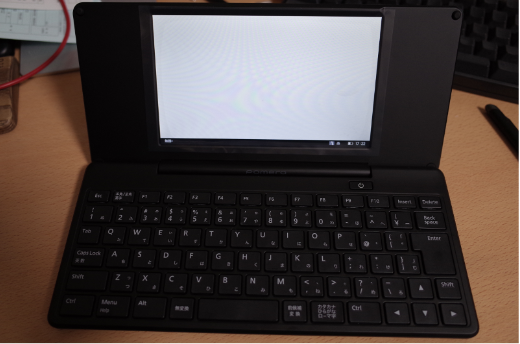
\includegraphics[scale=0.5]{image201709/dm200.png}
  \end{center}
\end{figure}

筆者はサイズ感が気に入っており、MD200をPCとして使えれば良かったのに、と感じました。

DM200のアップデータが公開されたときに、配布ファイルの構成がUbuntuではないかと話題になりました。実際に筆者がアップデータファイルの内容を確認してみると、パーティション情報がそのまま結合されて保存されているように感じ、DM200はLinuxベースなOSで動作しているのではないかと予想しました。

この考察からDM200をPCのように使えるかもしれないと考え、DM200を購入してDebian化に挑戦することにしました。


\subsection{DM200の解析}

\subsubsection{シリアルコンソールの場所}

DM200を普通に利用している状態では、Linuxの糸口を得ることができませんでした。そのため中身を開けてみて、組み込み機器用のデバッグ用シリアルコンソールを探してみました。基板を探してみると、すぐに見つかりました。

\begin{figure}[h]
  \begin{center}
    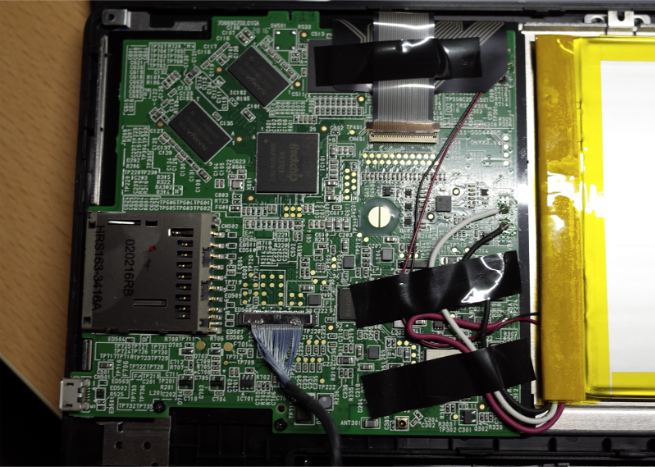
\includegraphics[scale=0.5]{image201709/dm200_board.png}
  \end{center}
\end{figure}


\begin{figure}[h]
  \begin{center}
    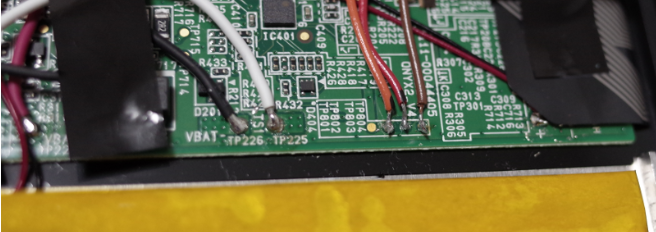
\includegraphics[scale=0.5]{image201709/dm200_board_serialconsole}
  \end{center}
\end{figure}

\subsubsection{ソースなしでがんばってみる}

実験として、描画プログラムをとめて、シリアルコンソールから/dev/fb0に適当なデータを書き込んでみました。するとDM200の画面になにやら描画されることを確認しました。そのため、chroot環境を作ってfbtermを使えば画面に描画処理ができるのではないかと考えました。

debianのchroot環境を作成するため、qemu-debootstrapを実行します。そして、できたrootfsをSDカードへコピーします。

\begin{commandline}
# qemu-debootstrap --arch=armhf --variant=minbase
\end{commandline}

SDカードをDM200に差し込み、DM200のシリアルコンソールからSDカード上のdebian rootfsへchrootします。chroot環境のfbtermを/dev/fb0指定で起動すると、内蔵の液晶画面に描画処理を行うことができました。


しかし、動作を確認するとキーリピートが効かない、画面左上が1文字だけ表示されないなど、多くの問題も見つかりました。


chroot環境で使うよりdebianなrootfsで起動してDM200を使いたいと考え、任意のrootfsで起動する方法を模索しました。組み込み機器ではU-Bootを使っている事例が多いため、DM200もU-Bootを使っているとすれば起動処理に割り込むことで任意のrootfsを起動できると推測しました。


\subsubsection{ソースコード開示請求}

ソースコードがない状況でU-Bootであるか推測しても解析が進まないため、お客様サポートフォームへ連絡し、DVDに収めたソースコード一式を入手しました。

ソースコードを調査し、以下が判明しました。

\begin{itemize}
\item U-Bootでの割り込み処理は無効になっている
\item kernel configはそのままではLCDにコンソールは出力できないように見える
\end{itemize}

Linuxのデスクトップ環境での利用を想定したkernel configではないことから、DM200のeMMCのU-Bootとkernelを書き換える必要があると考えました。


ただ、U-Bootの置き換えは失敗すると二度と起動しなくなる可能性があり(=文鎮化)、できることなら避けたい作業です。調査を進めるとU-Bootから呼び出せるkernelは2つあるようで、片方のkernelのみを書き換えるに留めた状態でどこまでdebianが動くか試してみることにしました。

\subsection{kernelのビルド}

\subsubsection{ビルド環境の構築}

DM200向けにkernelをビルドするため、コンパイルする環境が必要になります。まずはarmhfで動作する他のボード上でkernelをセルフコンパイルしてみましたが、とても遅い状態でした。\footnote{試したのはRaspberry Pi3(\url{https://www.raspberrypi.org/products/raspberry-pi-3-model-b/})、dragonboard(\url{https://developer.qualcomm.com/hardware/dragonboard-410c})。}\footnote{ビルド処理が遅いのはストレージが遅いためかもしれません。}

そこでqemu-debootstrapで作成したarmhf環境でkernelをビルドすることにしました。

\begin{commandline}
# qemu-debootstrap --arch=armhf --variant=buildd
\end{commandline}

この環境を使ってPC上でkernelのビルドを行うと5分程度で処理が終わります。


\subsubsection{kernel configの変更とkernelのビルド}

DM200のLCD上にコンソールを出力できるようにkernelの.configファイルへ以下を追加します。

\begin{commandline}
CONFIG_VT=y
CONFIG_VT_CONSOLE=y
CONFIG_HW_CONSOLE=y
CONFIG_FRAMEBUFFER_CONSOLE=y
\end{commandline}

また、U-Bootの書き換えを行わない方針のため、kernelの起動パラメータであるCMDLINEをU-Bootの現状の指定値から変更することができません。そのため、.configに必要なCMDLINEパラメータを指定します。

\begin{commandline}
CONFIG_CMDLINE="vmalloc=496M console=tty0  \
mtdparts=rk29xxnand:0x00002000@0x00002000(uboot), \
  : (snip)
,-@0x005FA000(reserve) \
rdinit=/sbin/init root=/dev/mmcblk0p15 storagemedia=emmc \
uboot_logo=0x02000000@0x7dc00000:0x01000000 \
loader.timestamp=2016-08-29_12:54:04 \
androidboot.mode=emmc loglevel=3 rootwait"
CONFIG_CMDLINE_FORCE=y
\end{commandline}


\subsection{rootfsの作成}

rootfsがどのように作られているかは、NetBSDを使っていたときにアーキテクチャ用のパッケージを展開しただけで動作していたことを思い出し、debootstrapで作成したディレクトリツリー一式をrootfsとしてそのまま使うことにしました。

rootfsを以下のコマンドで作成しSDカードへコピーしてDM200上で動作確認したところバイナリが動作することを確認しました。\footnote{Raspberry Piのrootfsの作成も同様にdebootstrapを使っているようです。\url{https://gist.github.com/abulte/3917357}}

\begin{commandline}
# qemu-debootstrap --arch=armhf --variant=minbase --include=XX
\end{commandline}


\subsection{rootfsの引き継ぎ}

Pomeraの標準環境のinitramfsから、SDカード上のdebootstrapで作成したrootfsへswitchすることができれば、debianが起動するはずです。しかし、switch\_rootはPID 1から実行できない制約があります。そのため、initramfsも作成することにしました。

initramfsはbusyboxで作成することができます。initramfsが展開されて最初に呼ばれる/sbin/initの処理に、switch\_rootを呼び出し、SDカード上のrootfsをmountし、mountしたSDカード内にあるinitを呼び出すようなスクリプトを作成しました。

これで、DM200がdebianとしてブートするようになりました。


\subsection{Debian化後の問題点}

\subsubsection{キーリピートが効かない}

キーリピートが効かない問題は、kernelのソースコード上で無効になっていたため、kernelのソースコードを修正しました。

\begin{commandline}
arch/arm/mach-rockchip/rk312x.c
static struct tc3589x_keypad_platform_data tc35893_data = {
  .krow = 8,
  .kcol = 12,
  .debounce_period = TC_KPD_DEBOUNCE_PERIOD,
  .settle_time = TC_KPD_SETTLE_TIME,
  .irqtype = IRQF_TRIGGER_FALLING  | IRQF_ONESHOT,
  .enable_wakeup = true,
  .keymap_data    = &onxy2_keymap_data,
  .no_autorepeat  = true, ←これ。falseに変更しました。
\end{commandline}

\subsubsection{ユーザーがネットワークを使えない}

以下のkernel configが有効の場合は特定のグループ以外からsocketが使えないと調べて判明しました。kernel configのパラメータを無効に変更してkernelをビルドし直すことで解消しました。

\begin{commandline}
CONFIG_ANDROID_PARANOID_NETWORK=y ←これをnに変更
\end{commandline}


\subsubsection{PomeraのROMとDebianで時刻がずれる}

DM200のRTCから取得した時刻は、Pomera標準のファームウェアではJSTとして扱っているようです。

今回作成したDebianなrootfsではRTCをUTCとして扱う設定になっていたため、Debian側でJSTとして認識させるように変更することで解消しました。


\subsubsection{USB-OTG機能が動かない}

ハード的に見るとIDラインが結線されていないため、自動認識は無理そうでした。

ソフトで強制的に有効にすると端末が死ぬことがわかり、ドライバをいじって無理やり何とかすることで対応しました。


\subsection{今後の課題}

DM200を実用するために以下の課題を解決していく必要があると思います。

\begin{itemize}
\item 内蔵GPU(MALI400)の有効化
\item USB-OTG 有効化時に死ぬ問題の調査
\item デバイスツリーの変更を行ってみる
\item suspend処理の見直し
\item 標準の高速起動処理を流用できないか
\item 他の起動方法ができないか調べてみる
\end{itemize}

\subsection{まとめ}

DM200をハックしてみました。

組み込み機器を解析する場合にはデバッグ用のシリアルコンソールを探してみるとよいでしょう。

また、GPLなソースコードは請求して中身を見てみるといろいろ勉強になり、ソースコードがあると自分で問題を対応できて楽しいです。

qemu-debootstrapは便利なコマンドですので覚えておくとよいと思います。


%
% 冊子にするために、4の倍数にする必要がある。
% そのための調整
\dancersection{メモ}{}
\mbox{}\newpage


\vspace*{15cm}
\hrule
\vspace{2mm}

\includegraphics[width=2cm]{image200502/openlogo-nd.eps}
\noindent \Large \bf Debian 勉強会資料\\
\noindent \normalfont \debmtgyear{}年\debmtgmonth{}月\debmtgdate{}日 \hspace{5mm}  初版第1刷発行\\
\noindent \normalfont 東京エリア Debian 勉強会 (編集・印刷・発行)\\
\hrule

\end{document}
